\documentclass[12pt,a4paper]{report}

\usepackage[utf8]{inputenc}
\usepackage[T1]{fontenc}
\usepackage[spanish]{babel}
\usepackage{geometry}
\usepackage{setspace}
\usepackage{titlesec}
\usepackage{hyperref}
\usepackage{graphicx}
\usepackage{float}
\usepackage{longtable}
\usepackage{array}
\usepackage{booktabs}
\usepackage[table]{xcolor}

\geometry{margin=2.5cm}
\onehalfspacing

\begin{document}

%-------------------------
% PORTADA
%-------------------------
\begin{titlepage}
\centering

```
\vspace*{2cm}

{\Huge\bfseries Análisis del Reto\par}

\vspace{2cm}

{\Large Plataforma de Distribución para ISBEN Solutions\par}

\vfill

\begin{flushright}
    Autores: Josué Pardo - Alberto Herrera\\
    Carrera: Computación\\
    Universidad: Universidad Técnica Particular de Loja\\
    Fecha: \today
\end{flushright}
```

\end{titlepage}

%-------------------------
% ÍNDICE
%-------------------------
\tableofcontents
\newpage

%-------------------------
% CAPÍTULO 1
%-------------------------
\chapter{Introducción}

\section{Introducción}
ISBEN Solutions es una empresa de software ubicada en Loja, Ecuador y planteo el reto de proponer una solución a las dificultades de las empresas de distribución en la ciudad, actualmente enfrentan múltiples contratiempos operativos relacionados con la gestión manual de pedidos, control de inventario, seguimiento de entregas y comunicación entre distribuidores, vendedores y propietarios de tiendas.
El proceso actual depende en gran medida de llamadas telefónicas, mensajes informales y registros manuales para verificar disponibilidad de productos, confirmar pedidos y coordinar entregas. Esta forma de trabajo genera retrasos, errores de comunicación y poca visibilidad del estado real de las operaciones.
Además, la empresa no dispone de una plataforma centralizada que permita controlar de forma eficiente el flujo completo de pedidos desde la creación hasta la entrega final.

\section{Problemática}
La situación actual se caracteriza por una gestión manual de pedidos basada en llamadas y mensajes informales, lo que deriva en pérdida de información, errores en registros y retrasos. Entre los problemas críticos identificados se encuentran:
\begin{itemize}
\item Falta de control de inventario en tiempo real: Los vendedores no conocen el stock disponible, provocando ventas de productos inexistentes.

\item Ausencia de trazabilidad: No existe claridad sobre quién crea, acepta o despacha un pedido, dificultando auditorías y resolución de reclamos.

\item Comunicación ineficiente: Dependencia excesiva de canales informales entre dueños de tiendas, vendedores y repartidores.

\item Falta de evidencia de entrega: Inexistencia de un registro formal o digital que valide la recepción de productos.

\item Escasa capacidad de monitoreo: Ausencia de reportes centralizados para la toma de decisiones estratégicas.
\end{itemize}

\section{Metodología o estrategia de desarrollo}
Para el desarrollo del sistema se adoptó la metodología ágil Scrum, debido a su enfoque iterativo e incremental, que permite entregar funcionalidades funcionales en períodos cortos de tiempo, recibir retroalimentación continua del cliente y adaptarse a cambios en los requisitos del proyecto.

El proyecto se desarrollará durante un período académico de 8 semanas, organizadas en sprints de una semana de duración. Al tratarse de un equipo de dos desarrolladores, ambos participan activamente en las actividades de análisis, diseño, desarrollo, pruebas y despliegue. Los roles de Product Owner y Scrum Master rotan entre los integrantes al inicio de cada sprint para garantizar la participación en todas las responsabilidades definidas por el marco Scrum.

Durante cada sprint se ejecutan las ceremonias principales de Scrum:

Sprint Planning: definición de objetivos y selección de elementos del Product Backlog.
Sprint Review: demostración de los incrementos desarrollados y recopilación de retroalimentación del cliente.
Sprint Retrospective: análisis de fortalezas, problemas y oportunidades de mejora para el siguiente sprint.



%-------------------------
% CAPÍTULO 2
%-------------------------
\chapter{Planificación y análisis}

\section{Análisis}
El análisis realizado en ISBEN Solutions permitió identificar diversas deficiencias en los procesos de gestión de pedidos, inventario y entregas. Actualmente, gran parte de las actividades operativas se ejecutan mediante procedimientos manuales o herramientas dispersas, lo que dificulta la coordinación entre distribuidores, vendedores, tiendas y personal de reparto. Esta situación genera retrasos en el procesamiento de pedidos, inconsistencias en los registros de inventario y una limitada capacidad para supervisar el estado de las operaciones en tiempo real.

La ausencia de una plataforma centralizada también afecta la trazabilidad de los procesos. La información se encuentra distribuida entre diferentes actores, dificultando el seguimiento de pedidos, la identificación de responsables ante incidencias y la generación de reportes confiables para la toma de decisiones. Asimismo, la falta de mecanismos automatizados de control incrementa el riesgo de errores humanos, duplicidad de información y pérdida de datos relevantes para la operación.

Desde la perspectiva del negocio, estas limitaciones reducen la eficiencia operativa y restringen la capacidad de crecimiento de la organización. La dependencia de procesos manuales incrementa los tiempos de respuesta, eleva los costos administrativos y afecta la calidad del servicio ofrecido a las tiendas y clientes finales.

Como resultado del análisis, se determinó la necesidad de implementar una plataforma web que centralice la gestión de usuarios, productos, inventario, pedidos y entregas. La solución propuesta permitirá automatizar actividades críticas, mejorar la comunicación entre los diferentes actores, proporcionar trazabilidad completa de las operaciones y disponer de información actualizada para el seguimiento y control del negocio.

La propuesta tecnológica responde directamente a los problemas identificados, incorporando mecanismos de autenticación y control de acceso por roles, gestión de inventario, seguimiento de estados de pedidos, confirmación digital de entregas mediante evidencia fotográfica y herramientas de monitoreo que faciliten la supervisión operativa. De esta manera, se espera mejorar la eficiencia de los procesos, reducir errores operativos y fortalecer la capacidad de gestión de ISBEN Solutions.



\section{Requisitos funcionales}

\textit{Nota metodológica: los requisitos funcionales que siguen fueron obtenidos por ingeniería inversa del código fuente actual del proyecto (\texttt{proyectoDistribuidora/}), no del diseño original. Reemplazan la versión anterior de esta sección, que describía un alcance más reducido (solo catálogo, inventario por vendedor y confirmación de entrega por fotografía). Varios de estos requisitos ya no corresponden exactamente al diseño inicial: el stock pasó de ser por vendedor (\texttt{VendorInventory}) a ser centralizado por bodega (\texttt{StockLevel} + bitácora \texttt{StockMovement}), la confirmación de entrega dejó de depender de una fotografía validada y ahora depende de la confirmación de la propia tienda, y se incorporó una capa completa de administración de la plataforma (multi-distribuidora, invitaciones, suspensión de cuentas) que no existía en el planteamiento original.}

\subsection{RF-01 --- Autenticación y sesión}

\begin{longtable}{|p{2cm}|p{2cm}|p{10cm}|}
\hline
\textbf{ID} & \textbf{Prioridad} & \textbf{Requisito} \\ \hline
RF-01.1 & M & El sistema debe autenticar usuarios mediante correo electrónico y contraseña; el correo es el identificador de inicio de sesión (no existe un nombre de usuario tradicional). \\ \hline
RF-01.2 & S & El inicio de sesión debe ofrecer una opción "recordarme": sin marcarla, la sesión expira al cerrar el navegador; marcada, se conserva según la vigencia por defecto de la sesión. \\ \hline
RF-01.3 & M & El sistema debe permitir solicitar la recuperación de contraseña mediante un enlace de un solo uso enviado al correo registrado. \\ \hline
RF-01.4 & M & El sistema debe permitir establecer una nueva contraseña usando un enlace válido, no utilizado previamente y no expirado (vigencia de 1 hora). \\ \hline
RF-01.5 & M & La respuesta a una solicitud de recuperación debe ser idéntica exista o no la cuenta asociada al correo, para evitar la enumeración de usuarios registrados. \\ \hline
RF-01.6 & M & El sistema debe invalidar la sesión del usuario al cerrar sesión. \\ \hline
RF-01.7 & S & Todo usuario autenticado debe poder cambiar su propia contraseña desde un panel de configuración personal, sin cerrar su sesión activa como efecto del cambio. \\ \hline
\end{longtable}

\subsection{RF-02 --- Control de Acceso Basado en Roles (RBAC) y aislamiento multi-tenant}

\begin{longtable}{|p{2cm}|p{2cm}|p{10cm}|}
\hline
\textbf{ID} & \textbf{Prioridad} & \textbf{Requisito} \\ \hline
RF-02.1 & M & El sistema debe soportar cinco roles: SUPER\_ADMIN (operador de la plataforma), DISTRIBUTOR, VENDOR, STORE\_OWNER y DELIVERY. \\ \hline
RF-02.2 & M & Cada vista debe validar el rol del usuario en el servidor: un usuario no autenticado es redirigido al inicio de sesión, y uno autenticado con un rol no autorizado recibe una respuesta 403 — nunca una redirección, para no revelar el rol observando a dónde es enviado. \\ \hline
RF-02.3 & M & Toda operación que modifique el estado de una entidad debe revalidar el rol de la sesión en el servidor; el cliente nunca debe ser una fuente confiable del rol del usuario. \\ \hline
RF-02.4 & M & Toda consulta de datos de negocio (productos, pedidos, inventario, tiendas, auditoría, etc.) debe filtrarse por la distribuidora del usuario autenticado; el aislamiento entre distribuidoras debe garantizarse a nivel de capa de datos, no solo de vista. \\ \hline
RF-02.5 & M & Únicamente el operador de la plataforma (SUPER\_ADMIN o superusuario) tiene visibilidad y acceso entre distribuidoras; ningún rol de negocio (DISTRIBUTOR, VENDOR, STORE\_OWNER, DELIVERY) puede ver información de una distribuidora distinta a la propia. \\ \hline
RF-02.6 & S & Si el operador suspende una distribuidora, el sistema debe bloquear el acceso operativo de todos sus usuarios (excepto a inicio/cierre de sesión), mostrando una pantalla de cuenta suspendida. \\ \hline
\end{longtable}

\subsection{RF-03 --- Administración de la plataforma (operador)}

\begin{longtable}{|p{2cm}|p{2cm}|p{10cm}|}
\hline
\textbf{ID} & \textbf{Prioridad} & \textbf{Requisito} \\ \hline
RF-03.1 & M & El operador debe poder visualizar un panel con todas las distribuidoras registradas, su estado (Activo / Suspendido / Prueba / Cancelado) y su plan (Gratis / Estándar / Premium). \\ \hline
RF-03.2 & M & El operador debe poder consultar el detalle de una distribuidora específica, incluyendo sus usuarios y sus últimas 20 entradas de auditoría. \\ \hline
RF-03.3 & M & El operador debe poder activar o suspender una distribuidora; cada acción debe quedar registrada en la auditoría con el operador responsable. \\ \hline
RF-03.4 & M & El operador debe poder dar de alta una nueva distribuidora junto con su primer usuario DISTRIBUTOR en una única operación atómica (todo o nada). \\ \hline
\end{longtable}

\subsection{RF-04 --- Autoregistro por invitación}

\begin{longtable}{|p{2cm}|p{2cm}|p{10cm}|}
\hline
\textbf{ID} & \textbf{Prioridad} & \textbf{Requisito} \\ \hline
RF-04.1 & M & El operador debe poder emitir una invitación de un solo uso, con vigencia de 7 días, para que una nueva distribuidora se autoregistre; si se indica un correo destino, el enlace se envía automáticamente. \\ \hline
RF-04.2 & M & El sistema debe rechazar una invitación de distribuidora que ya fue utilizada, revocada o expirada, informando el motivo específico de forma amigable. \\ \hline
RF-04.3 & M & El operador debe poder revocar una invitación pendiente en cualquier momento antes de ser canjeada. \\ \hline
RF-04.4 & M & Cada distribuidora debe contar con un enlace/token de invitación propio y regenerable para que nuevas tiendas se autoregistren, sin exponer públicamente la lista de distribuidoras existentes. \\ \hline
RF-04.5 & M & Al autoregistrarse una tienda mediante enlace de invitación, el sistema debe crear el usuario STORE\_OWNER y la tienda asociada en una sola transacción atómica, sin vendedor asignado (queda pendiente de que el distribuidor lo asigne). \\ \hline
\end{longtable}

\subsection{RF-05 --- Catálogo de Productos (DISTRIBUTOR)}

\begin{longtable}{|p{2cm}|p{2cm}|p{10cm}|}
\hline
\textbf{ID} & \textbf{Prioridad} & \textbf{Requisito} \\ \hline
RF-05.1 & M & El distribuidor debe poder crear productos indicando nombre, descripción, SKU (único por distribuidora), código de barras opcional, categoría, marca, unidad de medida, precio unitario y umbral de stock bajo. \\ \hline
RF-05.2 & M & El distribuidor debe poder editar la información de un producto existente. \\ \hline
RF-05.3 & M & El distribuidor debe poder desactivar o descontinuar un producto (estados Activo / Inactivo / Descontinuado); esto no elimina el registro ni afecta los pedidos ya existentes que lo referencian. \\ \hline
RF-05.4 & M & El distribuidor debe poder gestionar categorías, marcas y bodegas, cada una única dentro de su propia distribuidora. \\ \hline
RF-05.5 & S & El distribuidor debe poder asociar múltiples imágenes a un producto y marcar una de ellas como principal. \\ \hline
RF-05.6 & M & El distribuidor debe poder visualizar el catálogo completo con los precios vigentes (incluyendo descuentos activos). \\ \hline
\end{longtable}

\subsection{RF-06 --- Descuentos}

\begin{longtable}{|p{2cm}|p{2cm}|p{10cm}|}
\hline
\textbf{ID} & \textbf{Prioridad} & \textbf{Requisito} \\ \hline
RF-06.1 & S & El distribuidor debe poder crear un descuento por producto, definido como porcentaje o como monto fijo, acotado por una fecha de inicio y de fin. \\ \hline
RF-06.2 & M & El sistema debe impedir el solapamiento de dos descuentos para un mismo producto dentro de un mismo rango de fechas. \\ \hline
RF-06.3 & M & El precio con descuento debe calcularse dinámicamente sobre el precio base vigente en el momento de la consulta, sin almacenarse, y nunca debe resultar en un valor negativo. \\ \hline
\end{longtable}

\subsection{RF-07 --- Gestión de Inventario}

\begin{longtable}{|p{2cm}|p{2cm}|p{10cm}|}
\hline
\textbf{ID} & \textbf{Prioridad} & \textbf{Requisito} \\ \hline
RF-07.1 & M & El stock debe administrarse de forma centralizada por bodega (no por vendedor individual), siendo único por cada combinación producto + bodega. \\ \hline
RF-07.2 & M & El distribuidor debe poder registrar una recepción de mercancía (entrada positiva de stock) con motivo "Recepción". \\ \hline
RF-07.3 & M & El distribuidor debe poder registrar un conteo físico de inventario; el sistema debe calcular automáticamente la diferencia (delta) respecto al stock registrado. \\ \hline
RF-07.4 & M & El distribuidor debe poder registrar un ajuste manual de stock (mermas, correcciones), exigiendo obligatoriamente una nota que justifique el ajuste. \\ \hline
RF-07.5 & M & Todo movimiento de stock debe generar un registro inmutable en una bitácora de movimientos, incluyendo el saldo resultante después del movimiento, para permitir su reconciliación posterior. \\ \hline
RF-07.6 & M & El sistema debe impedir cualquier movimiento que deje el stock de un producto en una bodega con una cantidad negativa. \\ \hline
RF-07.7 & S & El distribuidor debe poder consultar el historial completo de movimientos de stock de un producto. \\ \hline
RF-07.8 & S & El distribuidor debe recibir una alerta cuando el stock total de un producto caiga por debajo de su umbral configurado (\texttt{low\_stock\_threshold}). \\ \hline
\end{longtable}

\subsection{RF-08 --- Importación de Productos vía CSV}

\begin{longtable}{|p{2cm}|p{2cm}|p{10cm}|}
\hline
\textbf{ID} & \textbf{Prioridad} & \textbf{Requisito} \\ \hline
RF-08.1 & S & El distribuidor debe poder importar productos de forma masiva desde un archivo CSV, mapeando categoría y marca por nombre. \\ \hline
RF-08.2 & M & El sistema debe sanitizar cada celda del archivo importado para neutralizar fórmulas potencialmente peligrosas (protección contra inyección de fórmulas / CSV injection). \\ \hline
RF-08.3 & M & Una fila inválida no debe impedir la importación del resto de filas válidas; el sistema debe reportar, por cada fila rechazada, su número y el motivo del rechazo. \\ \hline
\end{longtable}

\subsection{RF-09 --- Gestión de Tiendas}

\begin{longtable}{|p{2cm}|p{2cm}|p{10cm}|}
\hline
\textbf{ID} & \textbf{Prioridad} & \textbf{Requisito} \\ \hline
RF-09.1 & M & El distribuidor debe poder crear, editar y eliminar tiendas, y asignarles un vendedor responsable. \\ \hline
RF-09.2 & S & El propietario de una tienda debe poder editar los datos propios de su tienda (nombre, dirección, teléfono, ubicación), sin poder modificar su vendedor asignado ni su distribuidora. \\ \hline
RF-09.3 & S & El distribuidor debe poder visualizar un mapa con la ubicación geográfica de sus tiendas registradas. \\ \hline
\end{longtable}

\subsection{RF-10 --- Carrito y Creación de Pedidos (STORE\_OWNER)}

\begin{longtable}{|p{2cm}|p{2cm}|p{10cm}|}
\hline
\textbf{ID} & \textbf{Prioridad} & \textbf{Requisito} \\ \hline
RF-10.1 & M & El propietario de tienda debe poder explorar el catálogo de productos activos de su vendedor asignado, con filtro por categoría, antes de armar un pedido. \\ \hline
RF-10.2 & M & El sistema debe mantener el carrito de compras en la sesión del usuario, permitiendo agregar productos, editar cantidades y quitar líneas antes de confirmar el pedido. \\ \hline
RF-10.3 & M & Al confirmar el pedido, el sistema debe revalidar la disponibilidad de stock de cada línea; si alguna línea no puede cubrirse, el pedido no debe crearse y deben mostrarse los errores por línea, conservando el carrito intacto para su corrección. \\ \hline
RF-10.4 & M & El precio de cada línea del pedido debe fijarse (capturarse como snapshot) al momento de su creación, y no debe verse afectado por cambios posteriores en el precio del catálogo. \\ \hline
RF-10.5 & M & El propietario de tienda debe poder cancelar un pedido propio mientras se encuentre en estado Pendiente. \\ \hline
RF-10.6 & S & Si la tienda del usuario aún no tiene vendedor asignado, el sistema debe impedir la creación de pedidos e indicar que debe contactar al distribuidor. \\ \hline
\end{longtable}

\subsection{RF-11 --- Procesamiento de Pedidos (VENDOR)}

\begin{longtable}{|p{2cm}|p{2cm}|p{10cm}|}
\hline
\textbf{ID} & \textbf{Prioridad} & \textbf{Requisito} \\ \hline
RF-11.1 & M & El vendedor debe visualizar todos los pedidos en estado Pendiente asignados a él. \\ \hline
RF-11.2 & M & El vendedor debe poder aceptar un pedido pendiente; la aceptación debe ejecutarse en una única transacción atómica que bloquea las filas de stock involucradas, valida la disponibilidad de cada línea, descuenta el inventario y cambia el estado a Aceptado — todo o nada. \\ \hline
RF-11.3 & M & Si el stock es insuficiente para una o más líneas al momento de aceptar, la operación completa debe revertirse, el pedido debe permanecer en estado Pendiente, y debe informarse al vendedor el detalle del faltante por línea. \\ \hline
RF-11.4 & M & El vendedor debe poder rechazar un pedido pendiente, indicando opcionalmente un motivo que se notifica a la tienda solicitante. \\ \hline
RF-11.5 & M & El vendedor debe poder marcar como Despachado un pedido que se encuentre en estado Aceptado. \\ \hline
RF-11.6 & M & El panel del vendedor debe refrescar automáticamente la lista de pedidos pendientes mediante sondeo (polling) periódico, sin recargar la página completa; la cadencia del sondeo debe ser configurable por el propio vendedor (mínimo 10 segundos). \\ \hline
\end{longtable}

\subsection{RF-12 --- Entrega y Confirmación de Recepción}

\begin{longtable}{|p{2cm}|p{2cm}|p{10cm}|}
\hline
\textbf{ID} & \textbf{Prioridad} & \textbf{Requisito} \\ \hline
RF-12.1 & M & El personal de reparto debe visualizar todos los pedidos en estado Despachado de su distribuidora (sin asignación por ruta: el primero en llegar es quien confirma). \\ \hline
RF-12.2 & M & El personal de reparto debe poder confirmar una entrega, lo que cambia el estado del pedido a Entregado; opcionalmente puede adjuntar una fotografía como metadato de referencia, sin que esta sea obligatoria ni el sistema valide su origen o autenticidad. \\ \hline
RF-12.3 & M & El sistema debe impedir que un mismo pedido sea confirmado como entregado dos veces, incluso ante intentos simultáneos de distintos repartidores. \\ \hline
RF-12.4 & M & El propietario de tienda debe poder, sobre un pedido Entregado: confirmar la recepción (moviéndolo al estado final Confirmado) o reportar una incidencia describiendo el problema (moviéndolo a Problema de Entrega). \\ \hline
RF-12.5 & M & El vendedor o el distribuidor debe poder resolver una incidencia de entrega registrando notas de resolución; esto mueve el pedido al estado final Confirmado y notifica a la tienda. \\ \hline
\end{longtable}

\subsection{RF-13 --- Notificaciones}

\begin{longtable}{|p{2cm}|p{2cm}|p{10cm}|}
\hline
\textbf{ID} & \textbf{Prioridad} & \textbf{Requisito} \\ \hline
RF-13.1 & M & El sistema debe generar una notificación dentro de la aplicación ante cada cambio relevante de estado de un pedido (aceptado, rechazado, despachado, incidencia reportada, incidencia resuelta), dirigida al actor correspondiente. \\ \hline
RF-13.2 & M & Cada usuario debe poder marcar una notificación individual, o todas sus notificaciones, como leídas. \\ \hline
RF-13.3 & S & Cada usuario debe poder desactivar, por categoría (actualizaciones de pedido, alertas de stock bajo, alertas de nuevos pedidos), la generación de notificaciones dirigidas a él, sin afectar a los demás usuarios. \\ \hline
RF-13.4 & S & El distribuidor debe recibir un resumen de alertas de stock bajo tras cualquier operación que reduzca inventario o tras una importación CSV. \\ \hline
\end{longtable}

\subsection{RF-14 --- Panel Operativo y Auditoría del Distribuidor}

\begin{longtable}{|p{2cm}|p{2cm}|p{10cm}|}
\hline
\textbf{ID} & \textbf{Prioridad} & \textbf{Requisito} \\ \hline
RF-14.1 & M & El distribuidor debe visualizar un panel con el conteo de pedidos por estado, métricas resumidas de operación e inventario agregado por bodega. \\ \hline
RF-14.2 & M & El panel debe permitir filtrar los pedidos mostrados por rango de fechas, vendedor, tienda y estado, de forma combinable. \\ \hline
RF-14.3 & M & El distribuidor debe poder consultar el registro de auditoría de su propia distribuidora (acción realizada, entidad afectada, usuario responsable, estado previo/nuevo cuando aplique, y marca de tiempo), sin acceso a entradas de otras distribuidoras. \\ \hline
RF-14.4 & M & Toda transición de estado de un pedido, cambio de estado de un producto, movimiento de stock e invitación relevante debe generar automáticamente una entrada de auditoría, sin depender de una acción manual adicional. \\ \hline
\end{longtable}

\subsection{RF-15 --- API REST del Catálogo}

\begin{longtable}{|p{2cm}|p{2cm}|p{10cm}|}
\hline
\textbf{ID} & \textbf{Prioridad} & \textbf{Requisito} \\ \hline
RF-15.1 & M & El sistema debe exponer una API REST con operaciones CRUD para tiendas, productos, categorías, marcas, bodegas, niveles de stock, imágenes de producto y descuentos. \\ \hline
RF-15.2 & M & El acceso a la API debe requerir autenticación (por token o por sesión) y debe respetar el mismo aislamiento por distribuidora que la interfaz web. \\ \hline
RF-15.3 & S & El sistema debe exponer un endpoint independiente de sondeo para pedidos pendientes, separado de la API general del catálogo, destinado al refresco del panel del vendedor. \\ \hline
\end{longtable}

\section{Requisitos no funcionales}

\textit{Nota metodológica: a diferencia de la versión anterior de esta sección, los requisitos RNF-01, RNF-02 y RNF-03 que siguen describen garantías verificables directamente en el código fuente actual (mecanismos de bloqueo, transacciones atómicas, filtrado por distribuidora, estructura de la bitácora de auditoría). Los requisitos de RNF-04 relacionados con tiempos de respuesta y disponibilidad se mantienen como objetivos de diseño declarados por el equipo; a la fecha de este documento no existen pruebas de carga formales que los verifiquen, ya que la cobertura de pruebas automatizadas del proyecto se concentra en corrección funcional y seguridad de concurrencia, no en desempeño.}

\subsection{RNF-01 --- Seguridad}

\begin{longtable}{|p{2.5cm}|p{2cm}|p{9.5cm}|}
\hline
\textbf{ID} & \textbf{Prioridad} & \textbf{Requisito} \\ \hline
RNF-01.1 & M & Las contraseñas deben almacenarse mediante un hash criptográfico unidireccional; nunca en texto plano ni mediante cifrado reversible. \\ \hline
RNF-01.2 & M & El acceso a cualquier vista debe validarse en el servidor antes de renderizar contenido; el rol del usuario nunca debe inferirse ni confiarse desde el cliente. \\ \hline
RNF-01.3 & M & Toda operación que cambie el estado de una entidad debe revalidar en el servidor tanto el rol de la sesión como la pertenencia del recurso afectado a la distribuidora del usuario. \\ \hline
RNF-01.4 & M & Todas las consultas a base de datos sobre entidades de negocio deben incluir un filtro explícito por distribuidora; las fugas de datos entre distribuidoras deben ser estructuralmente imposibles, no evitadas únicamente por convención en cada vista. \\ \hline
RNF-01.5 & M & Los tokens de recuperación de contraseña y de invitación (de distribuidora o de tienda) deben ser de un solo uso, de vigencia limitada, y quedar inutilizables de forma permanente tras su consumo, expiración o revocación. \\ \hline
RNF-01.6 & S & Las respuestas del sistema a una solicitud de recuperación de contraseña no deben revelar si el correo ingresado corresponde o no a una cuenta registrada. \\ \hline
RNF-01.7 & S & Una distribuidora suspendida por el operador debe perder acceso operativo de forma inmediata para todos sus usuarios, sin necesidad de invalidar sesiones individualmente una por una. \\ \hline
\end{longtable}

\subsection{RNF-02 --- Integridad Transaccional y Concurrencia}

\begin{longtable}{|p{2.5cm}|p{2cm}|p{9.5cm}|}
\hline
\textbf{ID} & \textbf{Prioridad} & \textbf{Requisito} \\ \hline
RNF-02.1 & M & La aceptación de un pedido debe ejecutarse dentro de una única transacción atómica con bloqueo de filas sobre el stock involucrado, de modo que dos vendedores no puedan aceptar el mismo pedido ni descontar dos veces el mismo stock de forma simultánea. \\ \hline
RNF-02.2 & M & Toda mutación de una cantidad de stock debe pasar por un único punto de escritura centralizado que aplique el movimiento y su registro de auditoría de manera conjunta; no deben existir escrituras directas al campo de cantidad fuera de ese camino. \\ \hline
RNF-02.3 & M & La confirmación de una entrega debe ser resistente a intentos concurrentes: únicamente la primera confirmación válida debe surtir efecto; los intentos posteriores sobre el mismo pedido deben rechazarse de forma explícita. \\ \hline
RNF-02.4 & M & El canje de una invitación (de distribuidora o de tienda) debe ejecutarse dentro de una única transacción atómica que impida el doble registro con el mismo token. \\ \hline
RNF-02.5 & S & El sistema debe ofrecer una herramienta de reconciliación que compare el saldo almacenado de cada nivel de stock contra la suma de sus movimientos registrados, y reporte discrepancias por distribuidora. \\ \hline
\end{longtable}

\subsection{RNF-03 --- Auditoría y Trazabilidad}

\begin{longtable}{|p{2.5cm}|p{2cm}|p{9.5cm}|}
\hline
\textbf{ID} & \textbf{Prioridad} & \textbf{Requisito} \\ \hline
RNF-03.1 & M & Cada entrada de auditoría debe registrar como mínimo: usuario responsable de la acción, tipo de acción, tipo e identificador de la entidad afectada, estado previo y nuevo (cuando aplique) y marca de tiempo. \\ \hline
RNF-03.2 & M & El historial de movimientos de stock debe ser de solo-anexado (append-only); ninguna operación del sistema debe modificar o eliminar un movimiento ya registrado. \\ \hline
\end{longtable}

\subsection{RNF-04 --- Rendimiento}

\begin{longtable}{|p{2.5cm}|p{2cm}|p{9.5cm}|}
\hline
\textbf{ID} & \textbf{Prioridad} & \textbf{Requisito} \\ \hline
RNF-04.1 & M & Las vistas que listan entidades con relaciones (pedidos, notificaciones, auditoría) deben usar carga adelantada de relaciones; no se aceptan patrones de consulta N+1. \\ \hline
RNF-04.2 & M & Las tablas con alto volumen de consulta por estado o por relación (por ejemplo, pedidos por vendedor y estado, o por tienda) deben contar con índices compuestos dedicados. \\ \hline
RNF-04.3 & S & El endpoint de sondeo del panel del vendedor debe tener un costo acotado por solicitud (limitado a los pedidos pendientes propios del vendedor) y una cadencia mínima de 10 segundos entre solicitudes. \\ \hline
RNF-04.4 & S & El tiempo de respuesta de los endpoints de listado debe mantenerse perceptualmente inmediato ($\leq$ 500 ms) bajo el uso concurrente esperado para un piloto académico (decena de usuarios simultáneos); este objetivo es una meta de diseño, no un valor medido mediante pruebas de carga formales. \\ \hline
\end{longtable}

\subsection{RNF-05 --- Usabilidad}

\begin{longtable}{|p{2.5cm}|p{2cm}|p{9.5cm}|}
\hline
\textbf{ID} & \textbf{Prioridad} & \textbf{Requisito} \\ \hline
RNF-05.1 & S & Cada usuario debe poder personalizar qué categorías de notificación recibe y la cadencia de sondeo de su propio panel, sin alterar el comportamiento por defecto (todo activado) de los demás usuarios. \\ \hline
RNF-05.2 & S & Las validaciones de formulario deben mostrar errores específicos por campo, o por línea en el caso del carrito de compras, sin perder los datos ya ingresados por el usuario. \\ \hline
\end{longtable}


\section{Historias de Usuario / Casos de Uso}

Con el propósito de identificar las necesidades de los distintos actores involucrados en el sistema, se definieron historias de usuario basadas en la metodología ágil Scrum. Estas historias describen las funcionalidades que cada rol requiere para cumplir sus actividades dentro del proceso de gestión de pedidos, inventario y entregas.

\textit{Nota metodológica: la lista se actualizó por ingeniería inversa del código actual para reflejar capacidades que no existían en el planteamiento original (HU-22 a HU-30) y para corregir historias cuyo comportamiento cambió (HU-07 ya no es "asignar inventario a un vendedor", sino registrar movimientos de stock centralizado por bodega; HU-18 ya no depende de una fotografía obligatoria).}

\begin{longtable}{|p{2cm}|p{12cm}|}
\hline
\textbf{ID} & \textbf{Historia de Usuario} \\ \hline
HU-01 & Iniciar sesión en el sistema mediante correo electrónico y contraseña. \\ \hline
HU-02 & Cerrar sesión de forma segura. \\ \hline
HU-03 & Recuperar la contraseña mediante correo electrónico. \\ \hline
HU-04 & Crear nuevos productos en el catálogo. \\ \hline
HU-05 & Editar la información de productos existentes. \\ \hline
HU-06 & Desactivar o descontinuar productos del catálogo sin afectar pedidos existentes. \\ \hline
HU-07 & Registrar recepciones, conteos y ajustes de stock por bodega. \\ \hline
HU-08 & Consultar el dashboard operativo con información de pedidos e inventario. \\ \hline
HU-09 & Consultar la trazabilidad y auditoría de los pedidos. \\ \hline
HU-10 & Visualizar pedidos pendientes de procesamiento. \\ \hline
HU-11 & Aceptar pedidos y descontar inventario de forma segura. \\ \hline
HU-12 & Rechazar pedidos que no puedan ser atendidos. \\ \hline
HU-13 & Marcar pedidos como despachados. \\ \hline
HU-14 & Explorar el catálogo y armar un pedido mediante un carrito de compras. \\ \hline
HU-15 & Consultar el estado actual de los pedidos realizados. \\ \hline
HU-16 & Recibir notificaciones cuando cambie el estado de un pedido. \\ \hline
HU-17 & Visualizar los pedidos despachados asignados para entrega. \\ \hline
HU-18 & Confirmar la entrega de un pedido despachado. \\ \hline
HU-19 & Registrar automáticamente los movimientos de inventario para auditoría. \\ \hline
HU-20 & Registrar cambios realizados en el catálogo de productos. \\ \hline
HU-21 & Recibir alertas de inventario bajo umbral. \\ \hline
HU-22 & Confirmar la recepción de un pedido entregado o reportar una incidencia con lo recibido. \\ \hline
HU-23 & Resolver una incidencia de entrega reportada por una tienda. \\ \hline
HU-24 & Emitir y administrar invitaciones para el autoregistro de nuevas distribuidoras. \\ \hline
HU-25 & Autoregistrar una tienda mediante el enlace de invitación de una distribuidora. \\ \hline
HU-26 & Activar o suspender el acceso de una distribuidora como operador de la plataforma. \\ \hline
HU-27 & Gestionar descuentos por producto, acotados por fecha. \\ \hline
HU-28 & Importar productos masivamente desde un archivo CSV. \\ \hline
HU-29 & Personalizar las categorías y la cadencia de las notificaciones recibidas. \\ \hline
HU-30 & Consultar un mapa con la ubicación de las tiendas de la distribuidora. \\ \hline
\end{longtable}

\subsection{Casos de Uso }
Una vez identificadas las historias de usuario y las necesidades funcionales de los diferentes actores del sistema, se procedió a definir los casos de uso que describen de manera detallada la interacción entre los usuarios y la plataforma. Los casos de uso permiten especificar el comportamiento esperado del sistema, estableciendo las acciones que realiza cada actor, las condiciones necesarias para ejecutar un proceso, los posibles escenarios alternativos y los resultados obtenidos al finalizar cada operación.

\begin{longtable}{|p{2cm}|p{12cm}|}
\hline
\textbf{ID} & \textbf{Caso de Uso} \\ \hline
UC-01 & Iniciar Sesión \\ \hline
UC-02 & Cerrar Sesión \\ \hline
UC-03 & Recuperar Contraseña \\ \hline
UC-04 & Gestionar Catálogo de Productos \\ \hline
UC-05 & Registrar Recepción de Stock \\ \hline
UC-06 & Visualizar Panel de Operaciones \\ \hline
UC-07 & Consultar Registro de Auditoría \\ \hline
UC-08 & Gestionar Usuarios de la Plataforma \\ \hline
UC-09 & Visualizar Inventario por Bodega \\ \hline
UC-10 & Visualizar Pedidos Pendientes \\ \hline
UC-11 & Aceptar Pedido \\ \hline
UC-12 & Rechazar Pedido \\ \hline
UC-13 & Marcar Pedido como Despachado \\ \hline
UC-14 & Realizar Pedido desde el Carrito \\ \hline
UC-15 & Consultar Estado del Pedido \\ \hline
UC-16 & Visualizar Pedidos Despachados \\ \hline
UC-17 & Confirmar Entrega \\ \hline
UC-18 & Confirmar Recepción o Reportar Incidencia \\ \hline
UC-19 & Resolver Incidencia de Entrega \\ \hline
UC-20 & Emitir y Canjear Invitación de Distribuidora \\ \hline
UC-21 & Autoregistrar Tienda por Invitación \\ \hline
UC-22 & Activar o Suspender Distribuidora \\ \hline
\end{longtable}

\subsubsection{UC-01 -- Iniciar Sesión}

\begin{longtable}{|p{4cm}|p{10cm}|}
\hline
\textbf{Atributo} & \textbf{Descripción} \\ \hline
Actores & Operador, Distribuidor, Vendedor, Propietario de Tienda, Repartidor. \\ \hline
Precondiciones & El usuario dispone de una cuenta registrada y tiene asignado un rol dentro del sistema. \\ \hline
Flujo Principal &
1. El usuario accede a la pantalla de inicio de sesión.\\
& 2. Ingresa su correo electrónico y contraseña, y opcionalmente marca "recordarme".\\
& 3. El sistema valida las credenciales proporcionadas.\\
& 4. Se crea una sesión autenticada para el usuario, con la vigencia correspondiente según la opción "recordarme".\\
& 5. El sistema redirige al usuario al panel correspondiente a su rol. \\ \hline
Flujo Alternativo A1 & Si la contraseña es incorrecta, el sistema muestra un mensaje genérico de error y no inicia la sesión. \\ \hline
Flujo Alternativo A2 & Si la cuenta no existe, el sistema muestra el mismo mensaje genérico utilizado en el caso anterior para evitar revelar información sobre usuarios registrados. \\ \hline
Flujo Alternativo A3 & Si la distribuidora del usuario se encuentra suspendida, el sistema permite iniciar sesión pero bloquea el acceso a las funcionalidades operativas, mostrando una pantalla de cuenta suspendida. \\ \hline
Postcondiciones & El usuario dispone de una sesión activa y puede acceder a las funcionalidades autorizadas para su rol. \\ \hline
Requisitos Relacionados & RF-01.1, RF-01.2, RF-02.2, RF-02.6 \\ \hline
\end{longtable}
\subsubsection{UC-03 -- Recuperar Contraseña}

\begin{longtable}{|p{4cm}|p{10cm}|}
\hline
\textbf{Atributo} & \textbf{Descripción} \\ \hline
Actores & Distribuidor, Vendedor, Propietario de Tienda, Repartidor. \\ \hline
Precondiciones & El usuario tiene una dirección de correo electrónico registrada en el sistema. \\ \hline
Flujo Principal &
1. El usuario solicita la recuperación de contraseña ingresando su correo electrónico.\\
& 2. El sistema genera un token único con una vigencia de una hora.\\
& 3. Se envía un enlace de recuperación al correo registrado.\\
& 4. El usuario accede al enlace recibido.\\
& 5. El sistema valida que el token sea válido, no haya sido utilizado y no haya expirado.\\
& 6. El usuario registra una nueva contraseña.\\
& 7. El token queda marcado como utilizado. \\ \hline
Flujo Alternativo A1 & Si el enlace ya fue utilizado, el sistema informa que el enlace no es válido. \\ \hline
Flujo Alternativo A2 & Si el enlace ha expirado, el sistema solicita generar una nueva solicitud de recuperación. \\ \hline
Flujo Alternativo A3 & Si el correo no existe, el sistema muestra una respuesta idéntica a la del flujo exitoso, sin revelar la existencia de la cuenta. \\ \hline
Postcondiciones & La contraseña es actualizada y el usuario puede autenticarse utilizando la nueva credencial. \\ \hline
Requisitos Relacionados & RF-01.3, RF-01.4, RF-01.5 \\ \hline
\end{longtable}
\subsubsection{UC-04 -- Gestionar Catálogo de Productos}

\begin{longtable}{|p{4cm}|p{10cm}|}
\hline
\textbf{Atributo} & \textbf{Descripción} \\ \hline
Actores & Distribuidor. \\ \hline
Precondiciones & El usuario ha iniciado sesión y posee el rol de Distribuidor. \\ \hline
Flujo Principal &
1. El distribuidor accede al módulo de productos.\\
& 2. Registra un nuevo producto indicando nombre, descripción, SKU, categoría, marca, unidad de medida, precio unitario y umbral de stock bajo.\\
& 3. El sistema almacena la información asociándola al distribuidor correspondiente.\\
& 4. El producto aparece disponible dentro del catálogo, en estado Activo. \\ \hline
Flujo Alternativo A1 & El distribuidor modifica la información de un producto existente. Los cambios se reflejan en el catálogo sin afectar pedidos históricos, cuyos precios ya quedaron fijados al momento de crearse. \\ \hline
Flujo Alternativo A2 & El distribuidor desactiva o descontinúa un producto; el registro no se elimina y los pedidos que ya lo referencian no se ven afectados. \\ \hline
Flujo Alternativo A3 & Si faltan datos obligatorios o el SKU ya existe para esa distribuidora, el sistema muestra errores de validación y no registra el producto. \\ \hline
Postcondiciones & El catálogo queda actualizado y los productos pueden ser utilizados en los procesos posteriores del sistema. \\ \hline
Requisitos Relacionados & RF-05.1, RF-05.2, RF-05.3, RF-05.4 \\ \hline
\end{longtable}


\subsubsection{UC-05 -- Registrar Recepción de Stock}

\begin{longtable}{|p{4cm}|p{10cm}|}
\hline
\textbf{Atributo} & \textbf{Descripción} \\ \hline
Actores & Distribuidor. \\ \hline
Precondiciones & El producto existe y tiene un nivel de stock definido en al menos una bodega de la distribuidora. \\ \hline
Flujo Principal &
1. El distribuidor selecciona un producto.\\
& 2. Selecciona la bodega y el tipo de movimiento a registrar (recepción, conteo físico o ajuste).\\
& 3. Ingresa la cantidad correspondiente (y una nota, obligatoria en el caso de un ajuste).\\
& 4. El sistema calcula el nuevo saldo y crea el movimiento en la bitácora de stock.\\
& 5. El nivel de stock del producto en esa bodega queda actualizado de forma inmediata. \\ \hline
Flujo Alternativo A1 & Si el movimiento dejaría el stock en un valor negativo, el sistema rechaza la operación y muestra un mensaje de validación. \\ \hline
Flujo Alternativo A2 & Si se registra un ajuste sin indicar una nota, el sistema rechaza la operación. \\ \hline
Postcondiciones & El nivel de stock del producto en la bodega queda actualizado y el movimiento queda registrado de forma permanente en la bitácora. \\ \hline
Requisitos Relacionados & RF-07.2, RF-07.3, RF-07.4, RF-07.5, RF-07.6 \\ \hline
\end{longtable}
\subsubsection{UC-11 -- Aceptar Pedido}

\begin{longtable}{|p{4cm}|p{10cm}|}
\hline
\textbf{Atributo} & \textbf{Descripción} \\ \hline
Actores & Vendedor. \\ \hline
Precondiciones & El pedido existe, se encuentra en estado Pendiente y está asignado al vendedor autenticado. \\ \hline
Flujo Principal &
1. El vendedor visualiza un pedido pendiente.\\
& 2. Selecciona la opción Aceptar Pedido.\\
& 3. El sistema inicia una transacción de base de datos.\\
& 4. Se bloquean temporalmente los registros de stock involucrados para evitar conflictos concurrentes.\\
& 5. El sistema verifica que exista stock suficiente para todos los productos solicitados.\\
& 6. Se descuenta la cantidad correspondiente del stock, generando el movimiento respectivo en la bitácora.\\
& 7. El estado del pedido cambia a Aceptado.\\
& 8. El sistema registra el evento en la bitácora de auditoría y notifica a la tienda.\\
& 9. La transacción se confirma y los cambios quedan almacenados. \\ \hline
Flujo Alternativo A1 & Si alguno de los productos no dispone de stock suficiente, la transacción se revierte, el pedido permanece en estado Pendiente y se informa el motivo por línea al vendedor. \\ \hline
Flujo Alternativo A2 & Si dos vendedores intentan aceptar simultáneamente pedidos que compiten por el mismo stock, solo la primera operación válida se completa; las demás son rechazadas por falta de disponibilidad. \\ \hline
Postcondiciones & El pedido queda registrado como Aceptado, el stock se actualiza y se genera un registro de auditoría. \\ \hline
Requisitos Relacionados & RF-11.2, RF-11.3, RF-07.6, RF-14.4, RNF-02.1 \\ \hline
\end{longtable}


\subsubsection{UC-12 -- Rechazar Pedido}

\begin{longtable}{|p{4cm}|p{10cm}|}
\hline
\textbf{Atributo} & \textbf{Descripción} \\ \hline
Actores & Vendedor. \\ \hline
Precondiciones & El pedido existe, se encuentra en estado Pendiente y está asignado al vendedor autenticado. \\ \hline
Flujo Principal &
1. El vendedor consulta un pedido pendiente.\\
& 2. Selecciona la opción Rechazar Pedido e indica opcionalmente un motivo.\\
& 3. El sistema solicita confirmación de la acción.\\
& 4. El vendedor confirma el rechazo.\\
& 5. El estado del pedido cambia a Rechazado.\\
& 6. El sistema registra la acción en la bitácora de auditoría y notifica a la tienda, incluyendo el motivo si fue indicado. \\ \hline
Flujo Alternativo A1 & Si el vendedor cancela la confirmación, el pedido conserva su estado Pendiente. \\ \hline
Postcondiciones & El pedido queda marcado como Rechazado, sin afectar el stock disponible. \\ \hline
Requisitos Relacionados & RF-11.4, RF-14.4 \\ \hline
\end{longtable}


\subsubsection{UC-13 -- Marcar Pedido como Despachado}

\begin{longtable}{|p{4cm}|p{10cm}|}
\hline
\textbf{Atributo} & \textbf{Descripción} \\ \hline
Actores & Vendedor. \\ \hline
Precondiciones & El pedido se encuentra en estado Aceptado y pertenece al vendedor autenticado. \\ \hline
Flujo Principal &
1. El vendedor accede al detalle de un pedido aceptado.\\
& 2. Selecciona la opción Marcar como Despachado.\\
& 3. El sistema solicita confirmación de la acción.\\
& 4. El estado del pedido cambia a Despachado.\\
& 5. Se registra el evento en la bitácora de auditoría y se notifica a la tienda.\\
& 6. El pedido pasa a estar disponible para el personal de reparto. \\ \hline
Postcondiciones & El pedido queda en estado Despachado y puede ser gestionado por el personal de entrega. \\ \hline
Requisitos Relacionados & RF-11.5, RF-14.4 \\ \hline
\end{longtable}


\subsubsection{UC-14 -- Realizar Pedido desde el Carrito}

\begin{longtable}{|p{4cm}|p{10cm}|}
\hline
\textbf{Atributo} & \textbf{Descripción} \\ \hline
Actores & Propietario de Tienda. \\ \hline
Precondiciones & El usuario ha iniciado sesión como propietario de tienda y su tienda tiene un vendedor asignado. \\ \hline
Flujo Principal &
1. El usuario explora el catálogo de productos activos del vendedor asignado, con opción de filtrar por categoría.\\
& 2. Agrega productos y cantidades al carrito, guardado en su sesión.\\
& 3. Puede editar cantidades o quitar líneas antes de confirmar.\\
& 4. Envía la confirmación del pedido.\\
& 5. El sistema revalida la disponibilidad de stock de cada línea contra el nivel de stock vigente.\\
& 6. Se fija (snapshot) el precio vigente de cada producto al momento de la confirmación.\\
& 7. Se crea el pedido con estado Pendiente y se vacía el carrito.\\
& 8. El sistema confirma el registro exitoso del pedido y lo muestra al usuario. \\ \hline
Flujo Alternativo A1 & Si uno o más productos no tienen stock suficiente al confirmar, el pedido no se crea; se muestra el detalle de los errores por línea y el carrito se conserva intacto para su corrección. \\ \hline
Flujo Alternativo A2 & Si la tienda del usuario no tiene vendedor asignado, el sistema impide iniciar el carrito e indica que debe contactar al distribuidor. \\ \hline
Postcondiciones & El pedido queda registrado en estado Pendiente y disponible para revisión por parte del vendedor. \\ \hline
Requisitos Relacionados & RF-10.1, RF-10.2, RF-10.3, RF-10.4 \\ \hline
\end{longtable}


\subsubsection{UC-17 -- Confirmar Entrega}

\begin{longtable}{|p{4cm}|p{10cm}|}
\hline
\textbf{Atributo} & \textbf{Descripción} \\ \hline
Actores & Repartidor. \\ \hline
Precondiciones & El pedido se encuentra en estado Despachado. \\ \hline
Flujo Principal &
1. El repartidor accede al detalle de un pedido despachado.\\
& 2. Opcionalmente adjunta una fotografía de referencia (metadato no validado por el sistema).\\
& 3. Envía la confirmación de entrega.\\
& 4. El sistema verifica que el pedido siga en estado Despachado y no haya sido confirmado previamente por otro repartidor.\\
& 5. El estado del pedido cambia a Entregado, quedando pendiente de confirmación por parte de la tienda. \\ \hline
Flujo Alternativo A1 & Si el pedido ya fue confirmado por otro repartidor (condición de carrera), el sistema rechaza la operación e informa que ya no está disponible para confirmar. \\ \hline
Postcondiciones & El pedido queda registrado como Entregado; la confirmación final de recepción queda a cargo de la tienda (ver UC-18). \\ \hline
Requisitos Relacionados & RF-12.1, RF-12.2, RF-12.3 \\ \hline
\end{longtable}

\subsubsection{UC-18 -- Confirmar Recepción o Reportar Incidencia}

\begin{longtable}{|p{4cm}|p{10cm}|}
\hline
\textbf{Atributo} & \textbf{Descripción} \\ \hline
Actores & Propietario de Tienda. \\ \hline
Precondiciones & El pedido se encuentra en estado Entregado y pertenece a la tienda del usuario autenticado. \\ \hline
Flujo Principal &
1. El propietario de tienda revisa un pedido en estado Entregado.\\
& 2. Si lo recibido corresponde a lo solicitado, selecciona Confirmar Recepción.\\
& 3. El estado del pedido cambia al estado final Confirmado.\\
& 4. El sistema notifica al vendedor que la tienda confirmó la recepción. \\ \hline
Flujo Alternativo A1 & Si existe un problema con lo recibido, el propietario selecciona Reportar Incidencia y describe el inconveniente; el pedido cambia a estado Problema de Entrega y se notifica al vendedor y, si corresponde, al repartidor. \\ \hline
Postcondiciones & El pedido queda en estado Confirmado (cierre normal) o en Problema de Entrega, a la espera de resolución (ver UC-19). \\ \hline
Requisitos Relacionados & RF-12.4, RF-14.4 \\ \hline
\end{longtable}

\subsubsection{UC-19 -- Resolver Incidencia de Entrega}

\begin{longtable}{|p{4cm}|p{10cm}|}
\hline
\textbf{Atributo} & \textbf{Descripción} \\ \hline
Actores & Vendedor, Distribuidor. \\ \hline
Precondiciones & El pedido se encuentra en estado Problema de Entrega. \\ \hline
Flujo Principal &
1. El vendedor o el distribuidor revisa la incidencia reportada por la tienda.\\
& 2. Registra notas describiendo la resolución adoptada.\\
& 3. El estado del pedido cambia al estado final Confirmado.\\
& 4. El sistema registra la acción en la bitácora de auditoría y notifica a la tienda. \\ \hline
Postcondiciones & El pedido queda cerrado en estado Confirmado, con la incidencia y su resolución documentadas. \\ \hline
Requisitos Relacionados & RF-12.5, RF-14.4 \\ \hline
\end{longtable}


\section{Sprint}
El desarrollo del sistema se planificó mediante la metodología Scrum, organizando el trabajo en 8 sprints de una semana de duración cada uno. Cada sprint tiene como objetivo entregar un incremento funcional del producto, permitiendo validar avances de manera continua, identificar riesgos tempranamente y obtener retroalimentación para la planificación de las siguientes iteraciones.

Sprint 1 – Configuración del Entorno y Base del Proyecto.
Sprint 2 – Autenticación y Control de Acceso
Sprint 3 – Gestión de Catálogo
Sprint 4 – Gestión de Inventario
Sprint 5 – Gestión de Pedidos
Sprint 6 – Entrega y Auditoría
Sprint 7 – Dashboard y Funcionalidades Complementarias
Sprint 8 – Pruebas Integrales, Corrección de Incidencias y Despliegue	


\section{Diagramas: Clases y BD (diseño lógico) – Preguntas y respuesta al diagrama }

    \begin{figure}[H]
    \centering
    
\includegraphics[width=0.5\linewidth]{diagrama_de_clases.jpeg}
    \caption{Diagrama de Clases}
    \label{fig:clases}
\end{figure}
   

\subsection{Preguntas y respuestas del diagrama}
\begin{enumerate}
\item Pregunta 1. ¿Cómo garantiza el diseño del esquema el aislamiento de datos (multi-tenancy) para que diferentes distribuidoras no puedan acceder a la información de las demás?

La entidad Distributor actúa como eje central del modelo y se relaciona mediante la clave foránea distributorId con entidades como User, Store y Product. Gracias a esta estructura, todas las consultas pueden filtrarse por distribuidora, garantizando que cada organización únicamente acceda a sus propios usuarios, tiendas, productos y operaciones. Este enfoque permite cumplir con los requisitos de seguridad y confidencialidad, evitando fugas de información entre distribuidoras.

\item Pregunta 2. ¿Cómo puede determinarse qué distribuidora tiene el mayor volumen de ventas en un período determinado?

La consulta requiere relacionar las entidades Distributor, Store, Order y OrderItem. A través de la tienda se identifica la distribuidora propietaria, mientras que los ítems del pedido almacenan la cantidad vendida y el precio registrado en unitPriceAtTime. Esto permite calcular ingresos históricos reales por distribuidora, incluso cuando los precios actuales de los productos hayan cambiado posteriormente.

\item Pregunta 3. ¿De qué manera el esquema resuelve el problema de la pérdida de integridad en los precios históricos cuando el distribuidor actualiza el costo de un producto en el catálogo?

La solución se encuentra en la separación entre las entidades Product y OrderItem. Mientras Product almacena el precio actual del producto, OrderItem conserva el valor del campo unitPriceAtTime, registrando el precio exacto existente al momento de crear el pedido. De esta forma, los reportes históricos, facturación y análisis financieros permanecen consistentes aunque los precios del catálogo sean modificados posteriormente.

\item Pregunta 4. ¿Qué estructura permite al sistema controlar que un vendedor solo venda los productos y cantidades que tiene asignados?:

La entidad VendorInventory vincula a un usuario con rol vendedor (User) con un producto (Product) y una cantidad específica disponible. Esta tabla funciona como un inventario individual por vendedor, independiente del stock general de la distribuidora. Antes de aceptar una orden, el sistema puede verificar la existencia y disponibilidad en esta asignación, garantizando que el vendedor únicamente comercialice productos autorizados.

\item Pregunta 5. ¿Cómo permite el diagrama reconstruir la línea de tiempo completa de una orden que fue rechazada, modificada y procesada posteriormente?

Aunque la entidad Order conserva únicamente el estado actual del pedido, la trazabilidad histórica se obtiene mediante AuditLog. Esta entidad registra el usuario responsable (userId), la acción ejecutada (action), la entidad afectada (entityType), el identificador correspondiente (entityId) y detalles adicionales en formato JSON. Gracias a estos registros es posible reconstruir cronológicamente todos los eventos ocurridos sobre una orden, identificar responsables y realizar auditorías completas del proceso.



\end{enumerate}

\section{Diagrama de Componentes}

\begin{figure}[H]
    \centering
    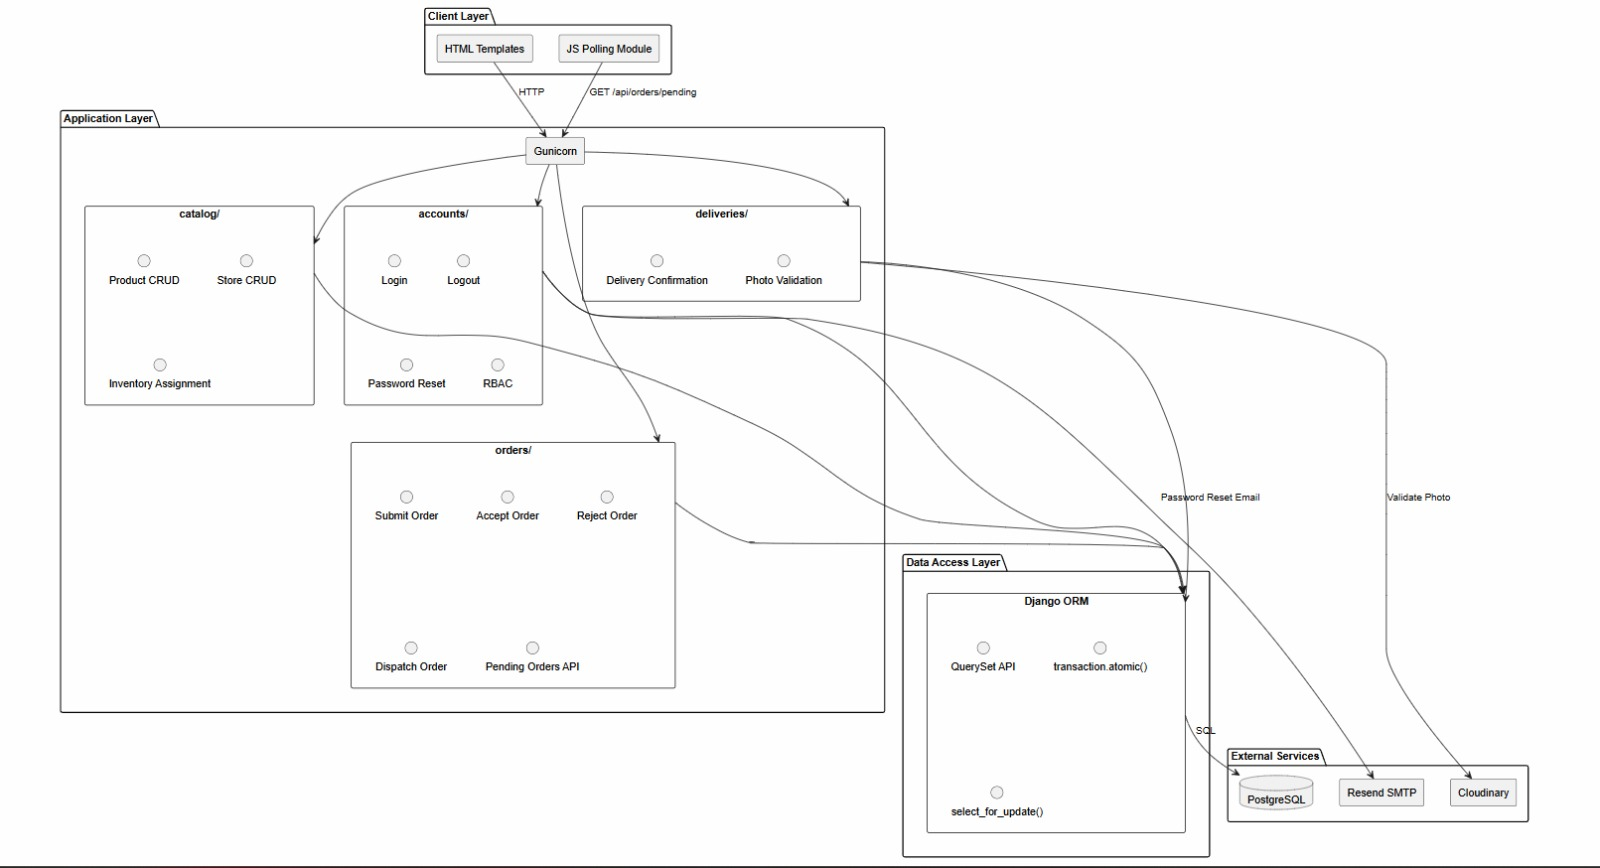
\includegraphics[width=\textwidth]{diagrama_componentes.jpeg}
    \caption{Diagrama de Componentes}
    \label{fig:componentes}
\end{figure}
La arquitectura del sistema se basa en un modelo de capas que promueve la separación de responsabilidades y facilita el mantenimiento, escalabilidad y seguridad de la aplicación. Las solicitudes de los usuarios se originan en la capa cliente, donde se presentan las interfaces web y se ejecutan mecanismos de actualización periódica mediante JavaScript. Estas solicitudes son procesadas por la capa de aplicación implementada con Django, la cual gestiona la autenticación, autorización basada en roles, validaciones de negocio y el flujo de las operaciones principales del sistema.

La capa de acceso a datos utiliza el ORM de Django para abstraer la comunicación con la base de datos PostgreSQL, garantizando la integridad transaccional, el aislamiento de datos entre distribuidoras y la optimización de consultas. Finalmente, la arquitectura integra servicios externos especializados para funciones complementarias, como el almacenamiento de evidencias fotográficas mediante Cloudinary y el envío de correos electrónicos a través de Resend. Esta organización permite desacoplar los componentes del sistema, mejorar la mantenibilidad del código y asegurar un flujo de comunicación controlado entre cada una de las capas.


\section{Arquitectura lógica y física (Propuesta)}

La arquitectura propuesta para el sistema ha sido diseñada con el objetivo de garantizar una adecuada separación de responsabilidades, facilitar el mantenimiento de la aplicación y permitir su crecimiento futuro sin afectar significativamente los componentes existentes. Para ello, se adopta una arquitectura multicapa basada en el patrón MVT (Model-View-Template) de Django, donde cada capa cumple una función específica dentro del procesamiento de las solicitudes y la gestión de la información.

Desde la perspectiva lógica, la solución organiza sus componentes en capas de presentación, aplicación, servicios transversales, dominio y acceso a datos. Esta estructura permite desacoplar la interfaz de usuario de la lógica de negocio y del almacenamiento de información, facilitando la implementación de mecanismos de seguridad, control de acceso basado en roles, auditoría de acciones y aislamiento de datos entre distribuidoras. Asimismo, favorece la reutilización de componentes y la mantenibilidad del sistema durante futuras fases de evolución.

Desde la perspectiva física, la arquitectura se apoya en una infraestructura basada en servicios en la nube. La aplicación se ejecuta sobre Railway utilizando Django y Gunicorn como plataforma de ejecución, mientras que PostgreSQL se emplea como sistema gestor de base de datos. Adicionalmente, se integran servicios externos especializados para el almacenamiento de evidencias fotográficas y el envío de correos electrónicos. Esta distribución permite aprovechar servicios administrados, reducir la complejidad operativa y mejorar la gestión operativa de la infraestructura mediante el uso de servicios administrados en la nube.-

La combinación de ambas arquitecturas proporciona una solución alineada con los requisitos funcionales y no funcionales del proyecto, garantizando seguridad, escalabilidad, mantenibilidad e integridad de la información, al tiempo que permite una comunicación eficiente entre usuarios, aplicación, base de datos y servicios externos.


\section{Prototipo de pantallas no funcional}
El diseño contempla dashboards específicos por rol:
Vista de Inventario: Niveles de stock visuales con alertas cuando el producto está bajo el umbral.
Dashboard de Pedidos: Lista con refresco automático cada 30 segundos (vía polling) para monitorear órdenes pendientes.
Interfaz de Entrega: Módulo de carga de archivos para la evidencia fotográfica del personal de reparto.
\subsection{Pantalla principal(Dashboard General del Distribuidor)}
La Figura 2.3 presenta el panel principal de operaciones del distribuidor dentro de la plataforma ISBEN Solutions. Esta interfaz ha sido diseñada para proporcionar una visión consolidada y en tiempo real de los principales indicadores operativos relacionados con la gestión de pedidos, inventario y recursos comerciales.
\begin{figure}[H]
    \centering
    
\includegraphics[width=0.5\linewidth]{image.png}
    \caption{Enter Caption}
    \label{fig:placeholder}
\end{figure}

\subsection{Pantalla de gestión (Gestión y Seguimiento de Pedidos de la Tienda)}
La Figura 2.4 presenta la interfaz de gestión de pedidos disponible para los propietarios de tiendas dentro de la plataforma ISBEN Solutions. Este módulo permite a los usuarios consultar el historial de pedidos realizados, monitorear su estado en tiempo real y generar nuevas solicitudes de abastecimiento de manera centralizada.
\begin{figure}[H]
    \centering
    
\includegraphics[width=0.5\linewidth]{image1.png}
    \caption{Enter Caption}
    \label{fig:placeholder}
\end{figure}
\subsection{Link del Prototipo en Replit}
https://ISBEN-distribution-hub--josuexpardoch.replit.app/
\end{document}
